Warning: truncated output (original token count: 10001)
Total output lines: 594

\documentclass[12pt,a4paper]{report}

\usepackage{fontspec}
\IfFontExistsTF{Times New Roman}
  {\setmainfont{Times New Roman}}
  {\setmainfont{Liberation Serif}}
\usepackage[a4paper,left=1.5in,right=1in,top=1in,bottom=1in]{geometry}
\usepackage{setspace}
\onehalfspacing
\usepackage{booktabs,tabularx,longtable,array}
\usepackage{enumitem}
\usepackage{xcolor}
\usepackage{graphicx}
\usepackage{caption}
\usepackage{float}
\usepackage{fancyhdr}
\usepackage{tikz}
\usetikzlibrary{arrows.meta,positioning,shapes.geometric}
\usepackage[numbers,sort&compress]{natbib}
\usepackage{hyperref}
\hypersetup{colorlinks=true,linkcolor=blue,citecolor=blue,urlcolor=blue}
\usepackage{titlesec}
\newcolumntype{Y}{>{\raggedright\arraybackslash}X}
\newcolumntype{L}[1]{>{\raggedright\arraybackslash}p{#1}}
\titleformat{\chapter}[hang]
  {\normalfont\bfseries\fontsize{14}{17}\selectfont}
  {Chapter \thechapter}{1em}{}
\titleformat{\section}
  {\normalfont\bfseries\fontsize{13}{16}\selectfont}
  {\thesection}{1em}{}
\titleformat{\subsection}
  {\normalfont\bfseries\fontsize{12}{14}\selectfont}
  {\thesubsection}{1em}{}
\titlespacing*{\chapter}{0pt}{-8pt}{18pt}
\setlength{\parindent}{0.3in}
\setlength{\parskip}{0pt}
\setlist{nosep,leftmargin=*}
\setcounter{secnumdepth}{3}
\setcounter{tocdepth}{2}
\renewcommand{\thefigure}{\thechapter.\arabic{figure}}
\renewcommand{\thetable}{\thechapter.\arabic{table}}
\captionsetup{font=small,labelfont=bf}
\pagestyle{fancy}
\fancyhf{}
\fancyhead[R]{Adaptive MoE Project Report}
\fancyfoot[C]{\thepage}
\renewcommand{\headrulewidth}{0.4pt}
\fancypagestyle{plain}{%
  \fancyhf{}\fancyhead[R]{Adaptive MoE Project Report}\fancyfoot[C]{\thepage}%
  \renewcommand{\headrulewidth}{0.4pt}}

\tikzset{
  block/.style={draw,rounded corners,align=center,text width=2.35cm,
    minimum height=1.05cm,font=\small,inner sep=4pt},
  smallblock/.style={draw,rounded corners,align=center,text width=2.1cm,
    minimum height=0.85cm,font=\footnotesize,inner sep=3pt},
  planned/.style={block,dashed},
  arrow/.style={-{Latex[length=2mm]},thick},
  plannedarrow/.style={-{Latex[length=2mm]},thick,dashed}
}

\begin{document}

%--------------------------- Title page ---------------------------
\begin{titlepage}
\thispagestyle{empty}
\centering
\vspace*{0.35in}
{\Large\bfseries PROJECT REPORT\par}
\vspace{0.55in}
{\LARGE\bfseries Adaptive Per-Expert Quantization for\\[0.15em]
Mixture-of-Experts Inference\par}
\vspace{0.4in}
{\large Project Status, Evidence Audit, and Research Roadmap\par}
\vspace{0.55in}
Submitted by\par
\vspace{0.15in}
\begin{tabular}{ll}
Varun Pandey & Roll number: IIT2024150\\
Chinmay Raheja & Roll number: IIT2024164\\
Sarthak Sharma & Roll number: IIT2024043
\end{tabular}
\vspace{0.45in}

Under the guidance of\par
Prof. Sonali Agarwal\par
\vspace{0.4in}
Department of Information Technology\par
Indian Institute of Information Technology Allahabad\par
Prayagraj, India\par
\vfill
November 2026
\end{titlepage}

\pagenumbering{roman}

%--------------------------- Certificate ---------------------------
\chapter*{Certificate}
\addcontentsline{toc}{chapter}{Certificate}
This is to certify that the project report entitled \textbf{Adaptive Per-Expert Quantization for Mixture-of-Experts Inference} has been prepared by Varun Pandey (IIT2024150), Chinmay Raheja (IIT2024164), and Sarthak Sharma (IIT2024043) under the guidance of Prof. Sonali Agarwal. The report is submitted as part of the Research Project course in the Department of Information Technology, Indian Institute of Information Technology Allahabad.

\vspace{1.0in}
\noindent
\begin{tabular}{cc}
\rule{2.4in}{0.4pt} & \rule{2.4in}{0.4pt}\\[-0.1em]
Project Guide & Head of Department\\
Name: Prof. Sonali Agarwal & Name: Prof. Vijay Kumar Chaurasiya\\
Date: 20 November 2026 & Date: 20 November 2026
\end{tabular}

%--------------------------- Declaration ---------------------------
\chapter*{Declaration}
\addcontentsline{toc}{chapter}{Declaration}
\textit{Draft declaration: verify this wording against institute policy and confirm each author's contribution before signing.}

We declare that this report presents the project work undertaken by the authors named on the title page. External papers, software, model documentation, and repository materials are cited. Results copied from saved project notebooks are identified as repository outputs and are not represented as independently reproduced measurements. Each author should review the final report and make any required corrections before signing.

\vspace{0.8in}
\begin{tabularx}{\linewidth}{X X}
Varun Pandey & Chinmay Raheja\\[0.35in]
Signature: \rule{2.1in}{0.4pt} & Signature: \rule{2.1in}{0.4pt}\\[0.2in]
Date: 20 November 2026 & Date: 20 November 2026\\[0.45in]
\multicolumn{2}{l}{Sarthak Sharma}\\[0.35in]
\multicolumn{2}{l}{Signature: \rule{2.1in}{0.4pt}\hspace{1.1in}Date: 20 November 2026}
\end{tabularx}

%--------------------------- Acknowledgement ---------------------------
\chapter*{Acknowledgement}
\addcontentsline{toc}{chapter}{Acknowledgement}
\textit{Replace this prompt with acknowledgements that reflect the team's actual guidance and contributions.}

The authors may acknowledge their project guide, department, teammates, and any infrastructure or dataset providers who materially supported the work. Names and contributions should be checked by the team before this page is finalized.

%--------------------------- Abstract ---------------------------
\chapter*{Abstract}
\addcontentsline{toc}{chapter}{Abstract}
This report documents an adaptive precision project for Mixture-of-Experts language-model inference. The project combines a Proximal Policy Optimization (PPO) policy with precision assignments for the 64 experts in OLMoE-1B-7B-0924. Its training notebook uses simulated battery, memory, energy, and thermal state; the policy observes 64 routing features and four resource features. The benchmark notebook evaluates prompt-token perplexity on 100 prompts. A code audit found that the benchmark's low-bit quantizers immediately dequantize their values and copy them into FP16 tensors. Its hybrid memory values are formula estimates, with a 32-layer default for a model whose published configuration has 16 layers. The saved outputs therefore provide exploratory evidence about quantization error and expert assignment, but do not demonstrate packed mixed-precision storage, measured memory savings, energy reduction, or live telemetry adaptation. At 100\% and 50\% battery, the saved PPO outputs have lower perplexity than the importance heuristic; at 10\%, PPO has higher perplexity than that heuristic. The report compares related work, reconstructs the prototype, specifies functional and non-functional requirements, describes the implemented replay-oriented user interface, and presents a test plan with current evidence and unmet checks. It recommends a follow-up study of measured device telemetry and task completion under hard resource limits. The proposed research direction is a hypothesis, not an established novelty claim.

\textbf{Keywords:} Mixture of Experts, language-model inference, mixed precision, quantization, PPO, hardware telemetry, task completion.

%--------------------------- Contents ---------------------------
\tableofcontents
\clearpage
\listoffigures
\addcontentsline{toc}{chapter}{List of Figures}
\clearpage
\listoftables
\addcontentsline{toc}{chapter}{List of Tables}
\clearpage
\chapter*{List of Abbreviations}
\addcontentsline{toc}{chapter}{List of Abbreviations}
\begin{tabularx}{\linewidth}{@{}lY@{}}
\toprule
Abbreviation & Meaning\\
\midrule
CUDA & Compute Unified Device Architecture\\
FP16 & 16-bit floating-point format\\
FP8 & 8-bit floating-point format\\
GPU & Graphics processing unit\\
HBM & High-bandwidth memory\\
INT8 & 8-bit integer quantization\\
KV & Key-value cache\\
LLM & Large language model\\
MLP & Multilayer perceptron\\
MoE & Mixture of Experts\\
NF4 & Normal Float 4-bit quantization\\
PPL & Perplexity\\
PPO & Proximal Policy Optimization\\
RAM & Random-access memory\\
VRAM & Video random-access memory\\
\bottomrule
\end{tabularx}
\clearpage

%--------------------------- Main report ---------------------------
\pagenumbering{arabic}

\chapter{Introduction}
\section{Background}
Large language models require substantial memory and compute. A Mixture-of-Experts model uses a router to select only a subset of expert networks for each token. This sparse computation reduces active work, while the weights for many experts still contribute to model storage requirements \citep{muennighoff2024olmoe}. Quantization reduces the number of bits used to represent weights, but aggressive compression can change model outputs. This project studies whether expert-level precision assignments can preserve useful model behavior under limited device resources.

\section{Problem statement}
The project aims to choose a precision tier for each expert using routing information and device state. The intended user benefit is to complete a language-model task within available memory, battery, thermal, and time budgets. The repository currently contains a PPO training simulator and a quantization-sensitivity benchmark. It does not yet demonstrate packed mixed-precision expert storage or a live controller driven by hardware sensors. This report therefore separates implemented code, saved notebook output, and proposed future work.

\section{Motivation}
Static precision applies the same format to every expert. A mixed assignment could reserve higher precision for experts that matter more to a request and use lower precision elsewhere. A resource-aware policy could also change its allocation as device conditions change. However, recent systems already investigate online expert precision and latency-aware allocation. A useful project contribution must therefore be evaluated against current methods and on actual hardware, with task outcomes as well as storage estimates.

\section{Objectives}
The project objectives are:
\begin{enumerate}
  \item Reconstruct the current PPO-based per-expert precision policy and its observation and reward definitions.
  \item Audit how the benchmark applies quantization and how it computes perplexity, memory, and energy-related values.
  \item Provide a transparent demonstration scaffold that does not present unmeasured values as hardware results.
  \item Define the engineering work and experiments required to test packed expert storage on a GPU.
  \item Formulate a candidate research question around measured device telemetry and user task completion.
\end{enumerate}

\section{Scope}
This report covers the BDA-IIITA repository's notebooks, model configuration, and demo scaffold \citep{adaptiveRepo,olmoeConfig}. It reviews saved output and source code; the notebook outputs have not been independently reproduced for this report. It does not claim a completed end-to-end runtime, packed mixed-precision GPU memory reduction, measured energy savings, or improved task success. The proposed research direction is explicitly prospective.

\section{Report organization}
Chapter 2 compares related work and states the candidate research gap. Chapter 3 presents requirements, feasibility, and technologies. Chapter 4 describes the architecture, data flow, controller procedure, and interface. Chapter 5 explains the repository modules and implementation challenges. Chapter 6 summarizes the test plan and saved results. Chapter 7 assesses the objectives and lists realistic future work.

\chapter{Literature Review}
\section{Related work}
HAQ uses reinforcement learning to select mixed-precision quantization policies with hardware feedback for latency and energy objectives \citep{wang2019haq}. DynaExq treats expert precision as an online allocation problem under a GPU memory budget and adapts precision using expert hotness \citep{chu2025dynaexq}. DyMoE combines expert orchestration and mixed-precision quantization for edge inference \citep{huang2026dymoe}. MatMoE dynamically selects expert bit widths from routing scores to meet changing latency constraints, making it especially close to the proposed project direction \citep{wei2026matmoe}. DynaMoE studies a neighboring problem: dynamic token-level expert activation and layer-wise capacity rather than quantized expert storage \citep{gulmez2026dynamoe}.

\section{Critical comparison}
Table~\ref{tab:literature} compares the cited systems by decision unit, resource information, and evidence relevant to this project. The comparison shows why generic claims about RL quantization or dynamic expert precision would not be sufficient.

\begin{table}[ht]
\centering
\small
\caption{Comparison of related systems and this project}
\label{tab:literature}
\begin{tabularx}{\linewidth}{@{}L{2.25cm}L{2.5cm}L{3.0cm}Y@{}}
\toprule
Work & Decision focus & Resource or policy signal & Relevance and distinction\\
\midrule
HAQ \citep{wang2019haq} & Layer bit-widths & Hardware feedback and resource objectives & Establishes RL-based hardware-aware mixed precision; not an MoE expert controller.\\
DynaExq \citep{chu2025dynaexq} & Online MoE expert precision & Expert hotness and HBM budget & Directly overlaps dynamic expert precision and memory-constrained serving.\\
DyMoE \citep{huang2026dymoe} & Expert orchestration and precision & Runtime edge inference signals & Shows that dynamic mixed-precision expert serving is an active direction.\\
MatMoE \citep{wei2026matmoe} & Dynamic expert bit-widths & Routing scores and changing latency target & Very close to routing-conditioned precision under changing system constraints.\\
DynaMoE \citep{gulmez2026dynamoe} & Active experts and layer capacity & Token complexity and layer schedule & Adjacent adaptive-capacity work; its central decision is expert activation.\\
Current project & 64 expert-index actions, shared across layers & Routing features plus simulated battery, RAM, drain, and thermal state & The benchmark returns low-bit values to FP16 tensors and estimates memory from assumed dimensions.\\
\bottomrule
\end{tabularx}
\end{table}

\section{Research gap and novelty boundary}
The current project should not claim to be the first use of RL for hardware-aware quantization or the first to adapt MoE expert precision. The literature already covers these broad ideas \citep{wang2019haq,chu2025dynaexq,huang2026dymoe,wei2026matmoe}. A narrower candidate question is whether directly measured external device telemetry, combined with task-completion outcomes and hard safety constraints, improves the probability of completing a user task over a session. This is a testable hypothesis, not a verified novelty result. Before making a publication claim, the team should compare the full methods and evaluations of the closest work, especially DynaExq and MatMoE.

\chapter{System Analysis and Requirements}
\section{Functional requirements}
The project has both an existing research prototype and a proposed live system. Table~\ref{tab:functional} separates functions already represented in the repository from functions that remain pending.

\begin{table}[ht]
\centering
\small
\caption{Functional requirements and current status}
\label{tab:functional}
\begin{tabularx}{\linewidth}{@{}L{1.1cm}Y L{2.2cm}Y@{}}
\toprule
ID & Requirement & Status & Evidence or remaining work\\
\midrule
FR-1 & Load routing features and construct PPO observations. & Implemented in notebook & 64 routing features and four simulated resource features.\\
FR-2 & Produce a three-tier action for 64 expert indices. & Implemented in notebook & One action vector is reused over model layers in the benchmark.\\
FR-3 & Compare precision assignments using model loss. & Exploratory & Saved prompt-token PPL output exists; hybrid storage is simulated.\\
FR-4 & Display or replay a run record in a web interface. & Scaffold present & Gradio UI and JSON/CSV record code exist; no validated GPU recording is bundled.\\
FR-5 & Retain packed expert weights at the selected precision. & Pending & The benchmark dequantizes to FP16; the live backend is gated.\\
FR-6 & Read live device telemetry and enforce a full-model budget. & Pending & Requires GPU instrumentation, calibration, and KV/workspace reservations.\\
FR-7 & Measure task completion and correctness. & Pending & The present benchmark measures prompt-token perplexity, not generated-task success.\\
\bottomrule
\end{tabularx}
\end{table}

\section{Non-functional requirements}
The intended runtime should be reproducible, resource-bounded, traceable, and safe to demonstrate. Every run should record the model revision, checkpoint hash, software versions, proposed and executed precision maps, changes made by the safety layer, timings, measurements, and correctness status. When a sensor or validated backend is unavailable, the interface should identify the missing evidence rather than show a fabricated result. Full-model inference should reserve memory for the KV cache and temporary workspaces and should reject assignments that exceed the calibrated budget.

\section{Feasibility study}
\subsection{Technical feasibility}
The repository contains a trained PPO checkpoint and an observation adapter. A single-expert gate has been added to check FP16, INT8, and NF4 module behavior on CUDA, but its output is not a full-model budget certification and the gate is not recorded as passed. The benchmark does not retain packed low-bit tensors. Thus, the proposed system is technically plausible, but live mixed-precision inference and its resource guarantees remain unverified.

\subsection{Operational feasibility}
The Gradio interface supports live-request controls in its layout and JSON-record replay. Its live backend currently fails closed, and no validated GPU recording is included. A reviewer can inspect the existing interface and replay records, but should not interpret the scaffold as a working adaptive inference service.

\subsection{Economic and schedule feasibility}
The project relies on open research software and an openly documente…1001 tokens truncated…ing controller};
\node[future,below=of controller] (packed) {Packed expert backend and budget guard};
\node[future,below=of packed] (task) {Generation and task-completion measurement};
\draw[plannedarrow] (telemetry) -- (controller);
\draw[plannedarrow] (controller) -- (packed);
\draw[plannedarrow] (packed) -- (task);
\end{tikzpicture}
\caption{Current notebook path (solid) and proposed live path (dashed)}
\label{fig:architecture}
\end{figure}

\section{Data-flow diagram}
Figure~\ref{fig:dataflow} shows the principal inputs and outputs. The training dataset and simulated state feed PPO; the benchmark applies assignments to a base model and stores saved metrics; the Gradio replay tab reads a JSON record. There is no validated data path from live sensors to full-model packed inference yet.

\begin{figure}[ht]
\centering
\resizebox{0.92\linewidth}{!}{%
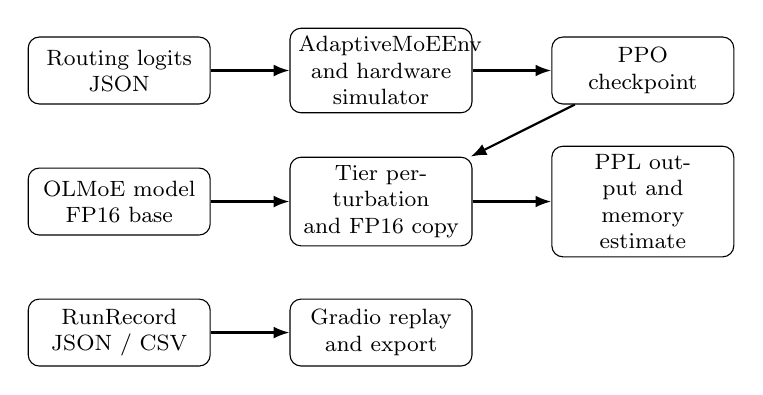
\begin{tikzpicture}[node distance=0.8cm and 1.0cm]
\node[smallblock] (rdata) {Routing logits\\JSON};
\node[smallblock,right=of rdata] (env) {AdaptiveMoEEnv\\and hardware simulator};
\node[smallblock,right=of env] (ppo) {PPO checkpoint};
\draw[arrow] (rdata) -- (env);
\draw[arrow] (env) -- (ppo);

\node[smallblock,below=of rdata] (model) {OLMoE model\\FP16 base};
\node[smallblock,right=of model] (perturb) {Tier perturbation\\and FP16 copy};
\node[smallblock,right=of perturb] (out) {PPL output and\\memory estimate};
\draw[arrow] (model) -- (perturb);
\draw[arrow] (ppo) -- (perturb);
\draw[arrow] (perturb) -- (out);

\node[smallblock,below=of model] (record) {RunRecord\\JSON / CSV};
\node[smallblock,right=of record] (ui) {Gradio replay\\and export};
\draw[arrow] (record) -- (ui);
\end{tikzpicture}}
\caption{Data flow through training, benchmark, and record replay}
\label{fig:dataflow}
\end{figure}

\section{Controller procedure}
The current training procedure is summarized below.
\begin{enumerate}
  \item Select a routing record and simulate battery, free RAM, drain rate, and thermal state.
  \item Standardize the 64 routing logits, compute expert importance, and append the four simulated state values.
  \item Ask PPO for one of three tier values for each of 64 expert indices.
  \item Calculate reward using fixed memory and energy costs and a surrogate quality penalty.
  \item In the benchmark, repeat the expert-index assignment across layers; quantize and dequantize selected weight values into FP16 tensors.
  \item Compute prompt-token perplexity and report a nominal memory estimate based on assumed bit widths.
\end{enumerate}

The observation and action interface can be written as:
\begin{verbatim}
importance = softmax(standardize(routing_logits))
obs = concatenate(64 * importance, simulated_telemetry)
action = PPO.predict(obs)
\end{verbatim}
This snippet describes the policy input/output contract. It does not implement physical mixed-precision storage.

\section{Record structure and data storage}
The demo does not use a relational database. Its run records are JSON objects and can be exported to JSON or CSV. Table~\ref{tab:record} lists the main fields represented by the \texttt{RunRecord} contract.

\begin{table}[ht]
\centering
\small
\caption{RunRecord data groups}
\label{tab:record}
\begin{tabularx}{\linewidth}{@{}L{3cm}Y@{}}
\toprule
Field group & Contents\\
\midrule
Request & Prompt, allocation choice, memory cap, battery scenario, and generation length.\\
Model and software & Model ID and revision, checkpoint hash, and package versions.\\
Assignments & Proposed and executed expert tiers and any safety adjustments.\\
Measurements & GPU identity, allocated/peak memory, latency, and other recorded values.\\
Correctness and events & Task correctness result plus timestamped status/error events.\\
\bottomrule
\end{tabularx}
\end{table}

\section{User-interface wireframe}
The source-defined interface has Live demo, Experts and resources, and Compare and evidence tabs. Figure~\ref{fig:ui} is a schematic of the controls in \texttt{demo/app.py}; it is not a runtime screenshot. The live gate is closed, so the interface does not present generated output or GPU measurements as available.

\begin{figure}[ht]
\centering
\fbox{\parbox{0.88\linewidth}{%
\textbf{Adaptive MoE: Quantization Lab}\par\smallskip
\textbf{Live demo tab}\par
Completion prompt: [text box]\par
Allocation: [uniform NF4 / INT8 / FP16 / heuristic / PPO]\par
Memory cap: [GiB] \quad Battery scenario: [100 / 50 / 10]\par
Maximum new tokens: [slider] \quad [Run] \quad [Stop]\par\medskip
\textbf{Status and output}\par
Streamed answer: unavailable while the gate is closed\par
Status: live inference unavailable\par
Measurements: none recorded \quad RunRecord: JSON\par\medskip
\rule{\linewidth}{0.4pt}\par\smallskip
Other tabs: Experts and resources; Compare and evidence (record upload/replay).}}
\caption{Source-based wireframe of the existing Gradio interface}
\label{fig:ui}
\end{figure}

\section{Design decisions and limits}
The current UI is designed to expose missing evidence rather than fill it with synthetic values. A future database schema is not applicable to the present branch because there is no database; the JSON record is the persistence contract. A future live system must additionally validate actual OLMoE layer and expert counts, preserve packed weights, reserve KV-cache/workspace memory, and record sensor availability. These are design requirements, not completed functions.

\chapter{Implementation}
\section{Training notebook}
The training notebook defines \texttt{AdaptiveMoEEnv}, a hardware simulator, and a PPO MLP with hidden widths 384 and 192. Each observation has 68 values and each action contains 64 tier choices. The reward combines estimated memory savings, estimated energy savings, a quality-loss proxy, and terminal survival terms. Training in the notebook specifies 200,000 timesteps and four vectorized environments. These quantities describe the saved training code, not physical resource savings.

\section{Benchmark notebook}
The benchmark evaluates 100 prompts across math, code, factual question answering, reasoning, and chat. It calculates loss over prompt tokens. The low-bit experiment rounds or quantizes weights and immediately dequantizes them to the source dtype before copying them to the FP16 tensors. The memory function uses nominal bits and fixed dimensions; it defaults to 32 layers and adds a fixed non-expert estimate. Therefore, benchmark outputs measure quantization perturbation on model logits and formula-derived storage estimates, not the memory of a packed mixed-precision model.

\begin{verbatim}
q4, state = quantize_4bit(weight, blocksize=64, quant_type="nf4")
weight_fp16 = dequantize_4bit(q4, state).to(weight.dtype)
expert_parameter.data[expert_id] = weight_fp16
\end{verbatim}
The code excerpt illustrates why this path does not retain packed NF4 weights.

\section{Demonstration modules}
The demonstration code is separated into the modules summarized in Table~\ref{tab:modules}. It includes a safe live-backend gate and replay support, but it does not yet connect the full model to a validated quantized runtime.

\begin{table}[ht]
\centering
\small
\caption{Main project modules}
\label{tab:modules}
\begin{tabularx}{\linewidth}{@{}L{2.4cm}Y L{2.8cm}@{}}
\toprule
Module & Responsibility & Current status\\
\midrule
Training notebook & \path{adapmoe-ipynb.ipynb}: PPO environment, policy diagnostics, and simulated hardware state. & Research prototype\\
Benchmark notebook & \path{adaptive-moe-real-benchmark.ipynb}: prompt-token loss and quantization-sensitivity comparisons. & FP16-backed simulation\\
Run-record contract & \path{demo/contracts.py}: RunRequest, RunEvent, and RunRecord structures. & Implemented\\
Policy adapter & \path{demo/policy.py}: checkpoint hash and observation/action compatibility. & Implemented; live run not established\\
Single-expert gate & \path{demo/expert_gate.py}: packed-format compatibility check. & Source present; validation not recorded\\
Inference backend & \path{demo/backend.py}: startup status and live inference entry point. & Fails closed pending validation\\
Replay and interface & \path{demo/replay.py} and \path{demo/app.py}: record loading/export and Gradio UI. & Replay scaffold present\\
\bottomrule
\end{tabularx}
\end{table}

\section{Challenges and resolutions}
Table~\ref{tab:challenges} records the main issues identified during the repository audit and the action taken or still required.

\begin{table}[ht]
\centering
\small
\caption{Implementation challenges and current handling}
\label{tab:challenges}
\begin{tabularx}{\linewidth}{@{}L{3cm}Y Y@{}}
\toprule
Challenge & Effect & Handling or next action\\
\midrule
Model configuration mismatch & README describes top-2 routing, while the selected configuration specifies 16 layers, 64 experts, and top-8. & Use model configuration as the source of truth in implementation and reporting.\\
Tier-name mismatch & Training labels use FP8/FP4; benchmark/demo labels use INT8/NF4. & Use an explicit canonical tier map and document quantizer semantics.\\
Simulated storage & Low-bit values return to FP16 tensors; memory is formula-based. & Keep results labelled as quantization simulation until packed storage is validated.\\
Policy input reuse & Benchmark allocation input comes from one routing record for multiple evaluation settings. & Profile request-specific routing features in future evaluation.\\
Live runtime validation & Full-model CUDA backend is unavailable behind a gate. & Run one-expert validation, then complete routing, memory, and failure-path checks on a GPU host.\\
\bottomrule
\end{tabularx}
\end{table}

\chapter{Testing and Results}
\section{Test plan and observed evidence}
Table~\ref{tab:tests} compares expected behavior with evidence available in the repository. A source-code check is not treated as a successful runtime test.

\begin{table}[ht]
\centering
\footnotesize
\caption{Test plan and current evidence}
\label{tab:tests}
\begin{tabularx}{\linewidth}{@{}L{1.0cm}L{3.0cm}Y Y@{}}
\toprule
ID & Test & Expected result & Actual evidence and status\\
\midrule
T-1 & Model configuration & Layer, expert, and top-k values read from the selected model config. & Published config indicates 16, 64, and top-8; README top-2 statement conflicts. Source fact checked; implementation must read config dynamically.\\
T-2 & Quantized parameter storage & INT8/NF4 weights remain packed after forward execution. & Benchmark dequantizes to FP16 and writes into FP16 expert tensors. Not passed.\\
T-3 & One-expert gate & Finite outputs, expected packed dtypes, FP16 comparison, and allocation ordering. & Gate source exists; no recorded GPU result. Not run or verified.\\
T-4 & Full-model resource guard & Real peak memory includes model, KV cache, and workspaces and respects budget. & Live backend remains gated; no full-model measurement. Not run.\\
T-5 & Task success & Generated output passes a domain-specific acceptance check. & Benchmark computes prompt-token PPL and does not generate task answers. Not measured.\\
T-6 & Replay and record parsing & Valid JSON record is displayed with output and event trace. & Replay code and UI handler are present; no validated GPU run record is bundled. Runtime result not established in this report.\\
T-7 & Energy and latency comparison & Direct device measurements for each allocation and task. & Mixed comparison table omits latency; training energy is simulated. Not measured.\\
\bottomrule
\end{tabularx}
\end{table}

\section{Saved perplexity and memory estimates}
Table~\ref{tab:results} reproduces the output saved in the benchmark notebook. The PPL column is the saved prompt-token loss result from a model forward pass after simulated quantization perturbations. The memory column is calculated from nominal bit widths and assumed tensor dimensions. Hybrid weights remain FP16 in this code path. Values are not independently reproduced for this report and have no reported confidence intervals.

\begin{table}[H]
\centering
\small
\caption{Exploratory benchmark output; memory is estimated, not measured for packed weights}
\label{tab:results}
\begin{tabularx}{\linewidth}{@{}Y>{\centering\arraybackslash}p{2.4cm}>{\centering\arraybackslash}p{2.0cm}>{\centering\arraybackslash}p{2.2cm}@{}}
\toprule
Configuration & \shortstack{Estimated expert\\memory (GB)} & \shortstack{Prompt-token\\PPL} & \shortstack{FP16/8-bit/NF4\\mix (\%)}\\
\midrule
Uniform FP16 & 25.77 & 13.0872 & 100/0/0\\
Uniform 8-bit proxy & 12.88 & 13.3455 & 0/100/0\\
Uniform NF4 proxy & 7.25 & 19.6175 & 0/0/100\\
PPO, battery 100\% & 14.97 & 13.2515 & 20.3/70.3/9.4\\
Importance heuristic, 100\% & 14.97 & 14.2392 & 20.3/70.3/9.4\\
PPO, battery 50\% & 14.51 & 13.2766 & 18.8/67.2/14.1\\
Importance heuristic, 50\% & 14.51 & 14.2169 & 18.8/67.2/14.1\\
PPO, battery 10\% & 12.95 & 18.6791 & 20.3/34.4/45.3\\
Importance heuristic, 10\% & 12.95 & 18.5626 & 20.3/34.4/45.3\\
\bottomrule
\end{tabularx}
\end{table}

At 100\% and 50\% battery, the saved PPO output has lower PPL than the importance heuristic. At 10\%, PPO has higher PPL than that heuristic. These outputs suggest that which expert receives a tier can affect loss, but the saved comparison does not show a consistent PPO advantage. No claim about task completion, packed storage, or user-facing speed follows from this table.

\section{Results interpretation}
The saved notebook contains an FP16 load result of 12.89 GiB allocated and 13.39 GiB peak for one run. This is separate from the all-FP16 formula estimate of 26.73 GB in the comparison table. The estimator defaults to 32 layers, although the selected model configuration has 16. It also adds 0.96 GB for non-expert parameters. Consequently, formula-derived memory cannot be used to claim a target-device fit.

The benchmark uses prompt tokens as labels and does not generate responses. Its PPL values measure token prediction loss under those prompts, not whether the model solved the math questions, generated correct code, or satisfied user intent. The report therefore treats the results as exploratory quantization-sensitivity evidence.

\chapter{Conclusion and Future Scope}
\section{Objectives and achievements}
Table~\ref{tab:objectives} summarizes progress against the objectives established in Chapter 1.

\begin{table}[ht]
\centering
\small
\caption{Objective status}
\label{tab:objectives}
\begin{tabularx}{\linewidth}{@{}Y L{2.4cm}Y@{}}
\toprule
Objective & Status & Evidence\\
\midrule
Reconstruct PPO policy and simulated state & Achieved for repository audit & Training notebook contains observation, action, reward, and simulator definitions.\\
Audit benchmark evidence & Achieved for repository audit & Quantize/dequantize path, PPL procedure, and memory estimator have been inspected.\\
Provide an honest demonstration scaffold & Partially achieved & Replay-oriented UI and run-record contracts exist; live backend is gated.\\
Validate packed mixed precision on a complete model & Not achieved & One-expert gate has no recorded result; full-model backend pending.\\
Demonstrate measured resource savings and task completion & Not achieved & Saved values do not include packed hybrid memory, live energy, or task-success evaluation.\\
\bottomrule
\end{tabularx}
\end{table}

\section{Conclusion}
The repository contains a PPO policy over 64 expert-index actions, a simulator for device state, saved prompt-token perplexity outputs, and a replay-first demonstration scaffold. The source audit shows that the mixed-assignment benchmark dequantizes low-bit values back into FP16 tensors and calculates memory from nominal bit counts. The available evidence is therefore preliminary and does not establish packed mixed-precision memory savings or live hardware adaptation. The result table shows that saved PPO PPL is lower than the importance heuristic at 100% and 50% battery, and higher at 10%.

\section{Future scope}
The recommended next work is to:
\begin{enumerate}
  \item Correct model-configuration and tier-name handling, and keep simulation metrics separate from physical measurements.
  \item Validate packed FP16, INT8, and NF4 expert modules on a CUDA host and record numerical error and allocation.
  \item Integrate a full-model backend that uses prompt-specific routing, measured telemetry, and a memory guard that includes KV cache and temporary workspaces.
  \item Compare static precision, importance heuristics, PPO, telemetry-only control, and combined routing-plus-telemetry policies on identical task inputs.
  \item Measure task success, latency, peak memory, energy, thermal behavior, and controller overhead with repeated runs and uncertainty estimates.
  \item Recheck novelty against DynaExq, DyMoE, and MatMoE before claiming a new method.
\end{enumerate}

\appendix
\chapter{Repository Artifacts and Run-Record Contract}
\section{Artifact map}
The project repository includes the PPO notebook, benchmark notebook, routing dataset, model checkpoint, and demo package. The demo package contains request/event/record contracts, policy preprocessing, a one-expert gate, a replay parser, and a Gradio app. No complete validated GPU run record is bundled with the demo scaffold.

\section{Run-record fields}
The \texttt{RunRecord} structure captures request settings, model identity and revision, checkpoint hash, software versions, proposed and executed assignments, safety adjustments, timings, measurements, correctness, and events. This record is the intended evidence unit for future runs. Every reported result should be traceable to such a record and to the exact source commit.

\section{Completion items for the team}
Before institutional submission, complete the roll numbers, department, guide, programme, certificate signatures, declaration wording, and acknowledgement. The current report is a structured project-status draft; the institution's thesis manual and supervisor's instructions take precedence over this generic BTech/MTech guide.

\bibliographystyle{IEEEtran}
\bibliography{references}

\end{document}
